
\begin{abstract} %Hier kommt eine Zusammenfassung des Projektes
	Es soll der Ladebereich eines LKWs aktiv gedämpft werden. Um das System simulieren zu können wird das System in Simulink nachgebaut. Anhand dieses Models soll nun 
	ein Regler entworfen und parametrisiert werden. Es soll ein digitaler Regler benutzt werden. 
	Hierfür muss noch zusätzlich ein Anti Aliasing Filter designt werden.
\end{abstract}

\begin{figure}[h] 
	\centering
		
\includegraphics[width=0.45\textwidth]{Bilder/truckIcon.jpg}
	\caption{kleiner LKW mit Laderaum}
	\label{SimulinkStreckenModell}
\end{figure}

\section{Einleitung}
Wenn der Laderaum eines Lkws voll geladen ist und über eine Landstraße bretter, dann kann es doch schon mal etwas holprig werden. Das ist nicht nur für den Fahrer unangenehm. Es kann auch gefährlich für den LKW und seine Ladung werden.
Eine zu hart eingestellte Federung kann Unebenheiten nicht ausgleichen, so wird die Ladung und das Fahrwerk nicht geschützt. Wenn die Federung zu weich eingestellt ist kann es 
wiederum zu schwingungen führen. Um dies zu vermeiden wird eine Dämpfung verwendet. Hierbei wird zusätzlich zu einer Feder mit der Federkonstanten $K$ ein Dämpfer mit der Dämpfungskonstanten $\mu$ verwendet. 
Diese beiden Parameter können nun genau auf die Masse $m$ des LKW und die zu erwartenden Unebenheiten abgestimmt werden. 
Wenn sich nun aber die Masse ändert, zum Beispiel beim be- und entladen, stimmt das Verhalten der Feder und des Dämpfers nicht mehr.
Da sich diese Parameter nicht einfach ändern lassen, wird ein aktives Dämpfungssystem verwendet. Hier wird zusätzlich zu der Feder und dem Dämpfer 
auch ein, meist pneumatischer aktuator verwendet. Der Aktuator soll störungen entgegenwirken und den Ladebereich auf einer Bestimmten höhe halten.
Die Kraft $F$ ist die Stellgröße in unserem Regelkreis.
	
\section{Ziele des Projekts}
In dieser Arbeit soll der Führungsfall betrachtet werden. Die höhe des Laderaums soll also so geregelt werden, dass Wunschhöhe $x_{w}$ während der laufzeit geändert werden kann.
In der Praxis kann diese Funktion beim Be- und Entladen nützlich sein. Oft haben Laderampen eine unterschiedliche Höhe. Der Bediener will den Ladebereich
beim Entladen auf die richtige Höhe einstellen können. Die Vorgabe soll sein, dass die Höhe $x$ auf 0 bis 1m eingestellt werden kann.

Der Laderaum soll während dem gesamten Entladeprozess die gleiche Höhe beibehalten, auch wenn die Masse geringer wird.
Ein Einschwingen ist zu vermeiden. Der LKW sollte nicht mit der Überdachung vor der Entladerampe kollidieren, also ist auch ein Überschwinger zu vermeiden.
Die Schnelligkeit des Einregelvorgangs steht in diesem Fall nicht im Vordergrund. Die Einregelzeit ist maßgeblich von der Kraft des Aktuators abhängig.
Diese sollte aus Kostengründen so groß wie nötig, aber so klein wie möglich dimensioniert werden. 
Es wird festgellegt, dass die Kraft des Aktuators (!! wie in Abb. dargestellt) nur nach oben wirkt. Aufgrund des Designs des pneumatischen Aktuators kann 
die Kraft nicht negativ werden.

Um diese Ziele zu erreichen, soll ein zeitdiskreter Regler mit den
richtigen Parametern entworfen werden. Dazu sind die
folgenden Schritte notwendig:

\begin{itemize}
	\item Nachbauen des Systems in Matlab Simulink
	\item Analysieren des Systems
	\item Dimensionieren eines Anti-Aliasing-Filters
	\item Bestimmung der Regelparameter mit Hilfe eines Parametrierverfahrens
	\item Optimieren der Regelparameter
\end{itemize}
	
\section{Theorie}

\subsection{Nachbauen des Systems}

\begin{figure*}[hbt] 
	\centering
		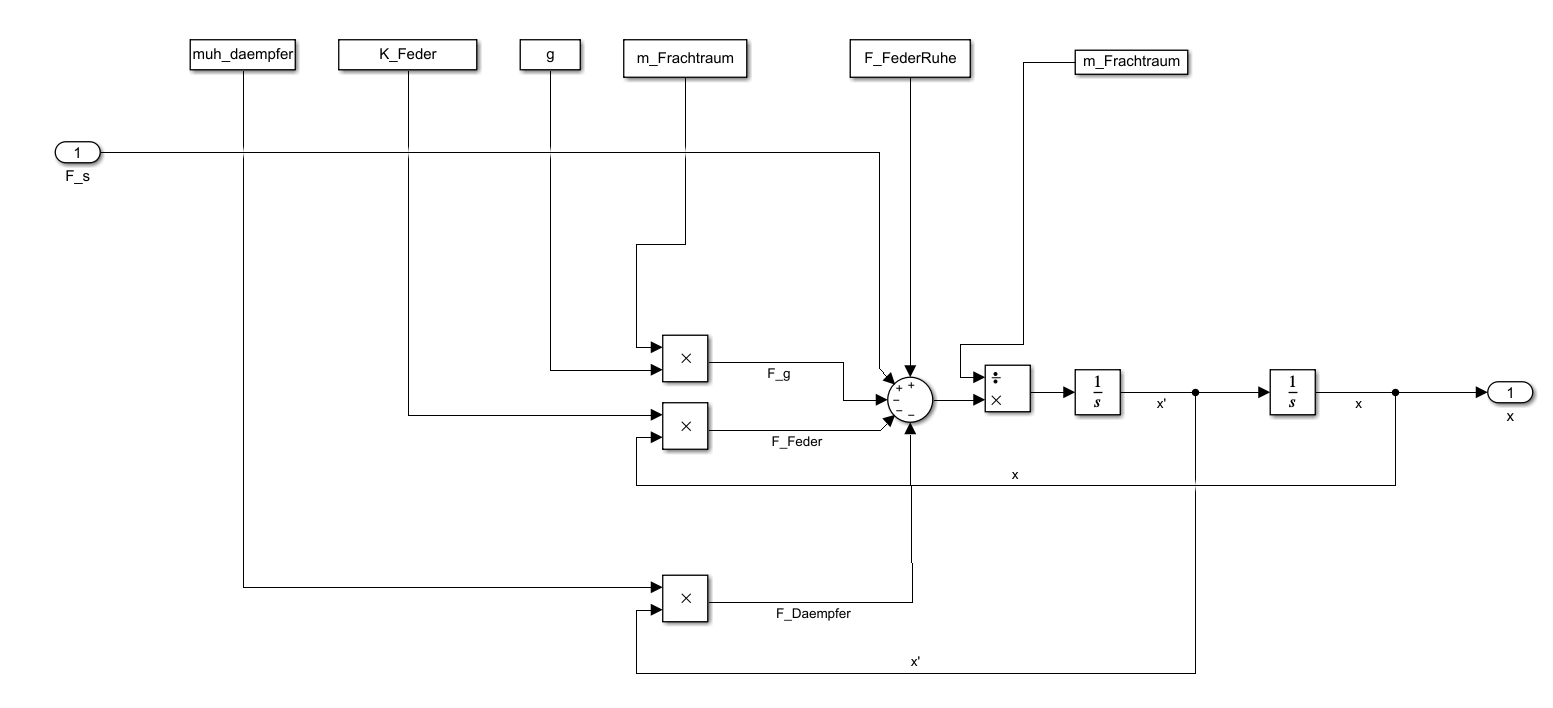
\includegraphics[width=1.0\textwidth]{Bilder/SimulinkStreckenModell.PNG}
	\caption{Simulink Modell der Regelstrecke}
	\label{SimulinkStreckenModell}
\end{figure*}

Als erster Schritt soll die zu regelnde Strecke in Simulink modelliert werden. Dafür muss zunächsteinmal die Differenzialgleichung aufgestellt werden.
Die Differenzialgleichung kann aus der Abbildung \ref{} abgeleitet werden. 
Nach dem Prinzip Aktio gleich Reaktio muss zu jedem Zeitpunkt ein Kräftegleichgewicht herrschen.
$x$ Entspricht der Höhe des Laderaums. Die positive x-Richtung zeigtnach oben. Die Feder wirkt mit der Kraft $F_{F} = K \cdot x$ nach oben. Der Dämpfer wirkt mit der Kraft 
$F_{R} = \mu \cdot \dot{x}$ entgegen der Bewegungsrichtung. Die Gewichtskraft $F_{G} = m \cdot g $ wirkt nach unten in negative x-Richtung. Der Pneumatik-Zylinder 
wirkt mit der Kraft  nach oben. Die Addition dieser Kräfte mit richtigem Vorzeichen ergibt die resultierende Beschleunigungskraft $F_{a} = m \cdot \ddot{x}$
in x-Richtung.

\begin{equation}
	m \cdot \ddot{x} = F_{S} + K \cdot x - \mu \cdot \dot{x} - m \cdot g
	\label{eq:Differenzengleichung}
\end{equation}

Für diese Formel muss angenommen werden, dass sich die Feder für alle realistischen Auslenkungen $\Delta x$ im linearen elastischen Bereich befindet. Wenn das System stillsteht ist $F_{a} = 0$ 
und $F_{R} = 0$. Damit ist $F_{F} = F_{g}$. Diese Stelle wird nun als $x = 0$ definiert. Durch diesen Trick kann $F_{g}$ weggelassen werden. 
Um die Gleichung in Simulink nachzubauen, wird sie nach ihrer höchsten Ableitung $a = \ddot{x}$ augelöst. Somit erhält man (\ref{eq:DifferenzengleichungAufgeloest}).

\begin{equation}
	\ddot{x} = \frac{F_{S} + K \cdot x - \mu \cdot \dot{x} - m \cdot g}{m}
	\label{eq:DifferenzengleichungAufgeloest}
\end{equation}

Wie in Abbildung \ref{SimulinkStreckenModell} dargestellt, ergibt sich $\dot{x}$ und $x$ durch das Integrieren von $\ddot{x}$.



$F_{g}$ und $F_{FederRuhe}$ heben sich eigentlich gegenseitig auf. Jedoch wurden sie in dem Simulink Modell gelassen,
um die Realität möglichst genau nachzubilden, und alle Freiheiten zu behalten.

\subsection{Analysieren des Systems}
Das Simulink Modell kann nun verwendet werden, um Das System zu analysieren.
Es soll die statische Verstärkung $K$, die Eigenfrequenz $\omega_{0}$ und die Dämpfung $d$ ermittelt werden.
Diese Werte lassen sich aus der Sprungantwort ablesen. Es wird ein Sprung von $F_{S} = \SI{1000}{N}$ 
auf das System gegeben. Die Sprungantwort sieht wie folgt aus.

\begin{figure}[h] 
	\centering
		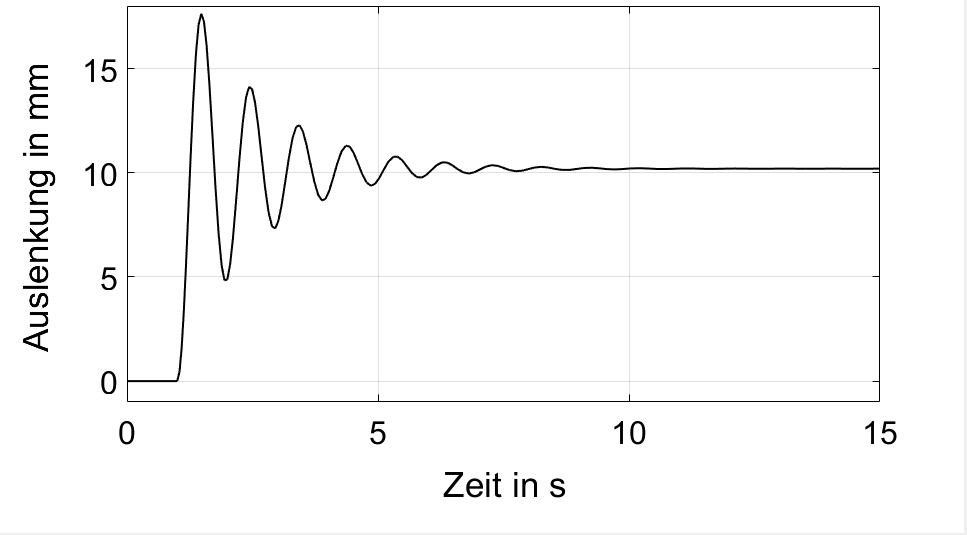
\includegraphics[width=0.45\textwidth]{Bilder/Stepresponse1000N.png}
	\caption{Sprungantwort auf 1000N}
	\label{SimulinkStreckenModell}
\end{figure}


Die statische Verstärkung ist definiert als: 

\begin{equation}
	\begin{split}
		K &=  \frac{Endwert ~ der ~ Sprungantwort}{Eingangssprung} = \frac{\SI{10,2}{mm}}{\SI{1000}{N}} \\
		\\
		&= \SI{10,2}{\frac{mm}{kN}} = \SI{1,02e-5}{ \frac{m}{N}}
		\label{eq:statischeVerstaerkung}
	\end{split}
\end{equation}


Der Endwert der Sprungantwort kann abgelesen werden, nachdem sich das System eingependelt hat.

Aus der Schwingung der Sprungantwort lässt sich die Eigenfrequenz ablesen. Für eine bessere Genauigkeit wird die Zeit $t$ für 
sechs Schwingungen mit einem Cursor gemessen. Die Eigenfrequenz berechnet sich dann wir folgt

\begin{equation}
	T = \frac{t}{6} = \frac{\SI{5,783}{s}}{6} = \SI{0,964}{s}
\end{equation}
\begin{equation}
	\omega_{0} = 2 \pi \cdot f = \frac{2 \pi}{T} = \frac{2 \pi}{\SI{0,964}{s}}  = \SI{6,52}{\frac{rad}{s}}
\end{equation}

Mithilfe der Formel aus \cite[Tabelle 9.8]{karlsruherPT2Glied} lässt sich die dämpfung aus der Sprungantwort berechnen:

\begin{equation}
	\begin{split}
		d &= \frac{\ln\Big(\frac{\Delta h_{1}}{\Delta h_{2}}\Big)}{\sqrt{4 \cdot \pi ^2 + \ln ^2 \Big(\frac{\Delta h_{1}}{\Delta h_{2}}\Big)}} \\
		\\
			&= \frac{\ln\Big(\frac{3,95}{2,1}\Big)}{\sqrt{4 \cdot \pi ^2 + \ln ^2 \Big(\frac{3,95}{2,1}\Big)}}
			= 0,1
	\end{split}
\end{equation}

Mithilfe dieser Werte und der Annahme, dass es sich um ein lineares PT2 Glied handelt, könnte man nun die Übertragungsfunktion (\ref{eq:Uebertragungsfunktion}) im Laplace-Bereich bilden.

\begin{equation}
	G(s) = \frac{x(s)}{F_{s}(s)} = \frac{K}{1 + 2 \cdot d \cdot T \cdot s + T^2 \cdot s^2}
	\label{eq:Uebertragungsfunktion}
\end{equation}
Aber die brauchen wir jetzt eigentlich gar nicht mehr.


\subsection{Interpretation der Werte}\label{subSec:Interpraetation}
Aus der statischen Verstärkung $K$ ist zu erkennen, dass eine Große Kraft nötig ist, um die Ladefläche zu bewegen. Mit der Formel (\ref*{eq:statischeVerstaerkung}) kann ausgerechnet werden, welche Kraft nötig 
ist, um $x = \SI{1}{m}$ zu erreichen.

\begin{equation}
	F_{s}= \frac{x_{max}}{K}  = \frac{1}{\SI{1,02e-5}{ \frac{m}{N}}} = \SI{98}{kN}
\end{equation}

Der Laderaum soll mit vier einfachwirkenden Hydraulikzylindern gesteuert werden. 
Ein passender Zylinder sollte einen Hub von circa $\SI{1,5}{m}$ haben.
Die vier Zylinder sollten eine Gemeinsame Kraft von mindestens $F = \SI{50}{kN}$ aufweisen.
Es werden Zylinder ähnlich dem in \cite{Zylinder} zum Einsatz kommen.
Jeder Zylinder hat einen Hub von $\SI{1,5}{m}$
und eine Kraft von $F = \SI{1000}{kN}$. Damit ist das Stellglied auf eine Maximalkraft von 
\begin{equation}
	F_{s, max} = 4 \cdot \SI{1000}{kN} = \SI{4000}{kN}
\end{equation}
begrenzt. Es bleibt also noch genug Kraft übrig, um Regeln zu können.
In der Praxis sollte die Kraft so beschränkt werden, dass die Fracht eine maximal Beschleunigung von circa $0,5g$ erfährt.
Für sie Simulation wird keine Beschränkung für das Stellglied festgellegt.

\section{Reglerentwurf}

\subsection{Digitalisierung und Antialiasing}
Die Höhe des Laderaums wird durch einen Sensor ausgelesen. Das Signal dieses Sensors soll digitalisiert werden.
Für die digitalisierung wird ein Sample and hold Glied benutzt. Vor dieses Glied muss ein Anti aliasing Filter eingebaut werden.
Nun soll die Samplefrequenz und die Grenzfrequenz festgellegt werden. Im letzten Abschnitt wurde die Eigenfrequenz bereits zu $\SI{6,52}{\frac{rad}{s}}$ bestimmt.
Die Abtastrate sollte nach \cite{NotholtVorlesung5} das zehn bis zwanzigfache der schnellsten
Zeitkonstanten betragen. 

\begin{equation}
	f_{s} = \frac{\omega_{0}}{2 \pi} \cdot 20 = \SI{20,75}{Hz}
\end{equation}

Eine Abtastfrequenz von $\SI{20,75}{Hz}$ reicht also aus um das System vernünftig regeln zu können. Diese Frequenz ist recht gering.
Selbst die günstigsten Analog to Digital Converter (ADC) erreichen viel höhere Abtastraten. 
Generell gilt, dass eine geringere Abtastfrequenz eine erhöhte Verzögerung des Signals nach sich zieht. Eine erhöhte Verzugszeit $T_{u}$
erschwert das Regeln. Daher sollte die Abtastfrequenz möglichst hoch gewählt werden. Solange die Auflösung des ADC nicht darunter leidet.
Falls der verwendete Sensor hochfrequente Störungen hat, welche größer als eine Stufe des ADC sind, kann versucht werden diese Störungen durch 
einen Tiefpassfilter herauszufiltern.

In der Simulation ist der x-Wert Störungsfrei, also könnte die Abtastfrequenz beliebig hoch gewählt werden.
Für diesen Versuch wird sich aber auf eine relativ moderate Frequenz von 

\begin{equation}
	f_{s} = \SI{10}{kHz}
\end{equation}

beschränkt.

Da es wie schon erwähnt in dieser Simulation keine Störungen gibt, wäre kein Anti-Aliasing-Filter notwendig. Er sollte in diesem Fall sogar vermieden werden,
da er eine Verzugszeit mit sich bringt.
Der Anti-Aliasing-Filter ist Teil der Anforderungen also wird nachfolgend trotzdem einer verwendet.
Die Aufgabe des Anti-Aliasing-Filter ist es die Einhaltung des Nyquist-Shannon-Abtasttheorems sicherzustellen. Der Tiefpass soll alle Frequenzen, 
größer als $f_{S} / 2$ herausfiltern. Um dies sicherzustellen wird die Grenzfrequenz auf

\begin{equation}
	f_{G} = \frac{f_{S}}{4} = \SI{2,5}{kHz} 
\end{equation}

festgellegt. Diese doppelte Sicherheit ist möglich, da bei der Abtastfrequenz viel Spielraum gelassen wurde. Es ist zu empfehlen einen Filter höherer Ordnung zu 
wählen. Für diese Arbeit wird einfachheitshalber ein Tiefpass 1. Ordnung verwendet.
Für die Zeitkonstante des Filters ergibt sich:

\begin{equation}
	T_{F} =  \frac{1}{f_{G}} = \frac{1}{\SI{2.5}{kHz}} = \SI{0,4}{ms}
\end{equation}


\begin{figure*}[hbt] 
	\centering
		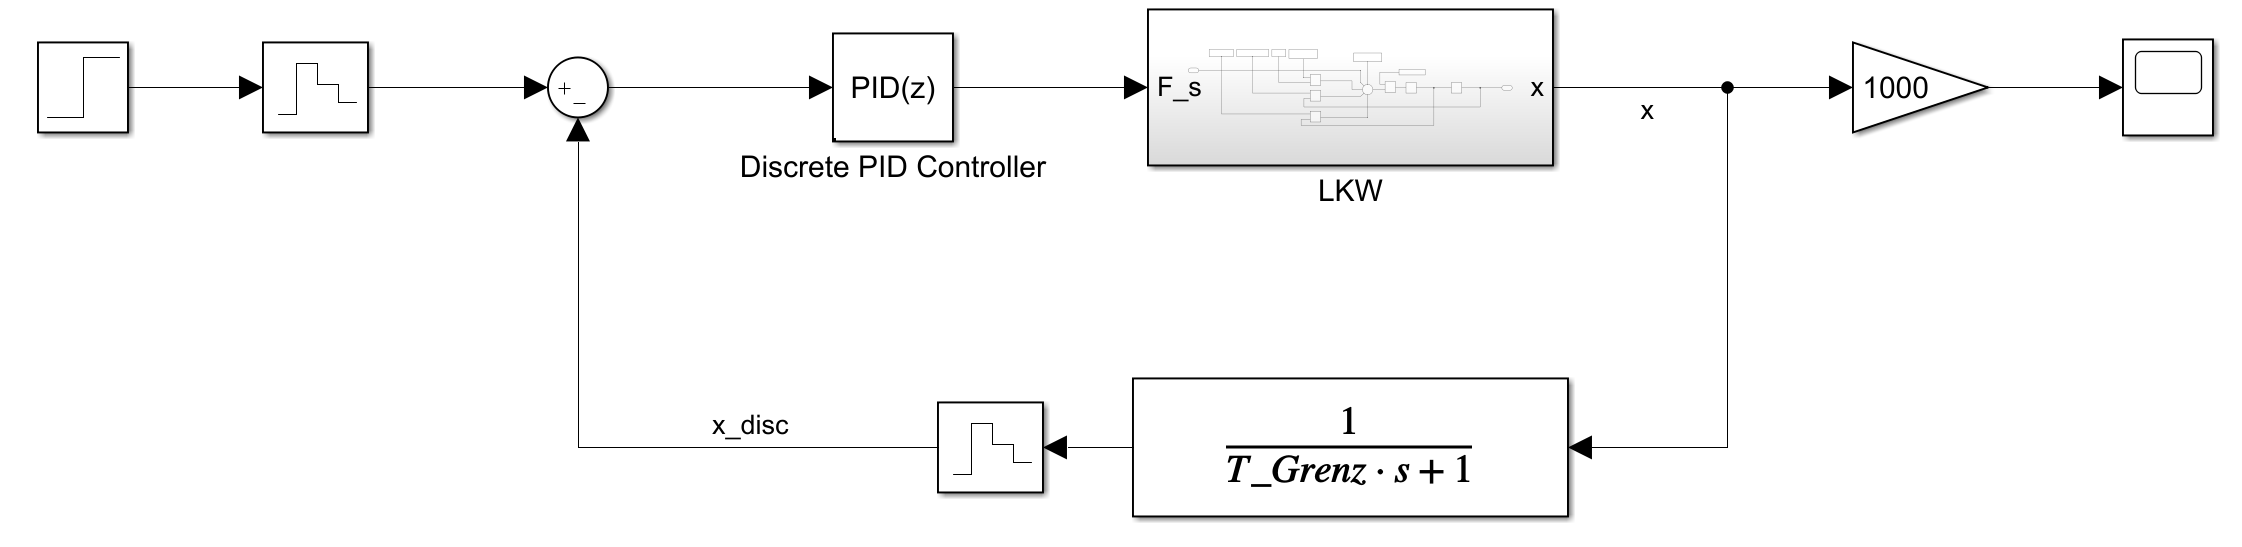
\includegraphics[width=1.0\textwidth]{Bilder/geschlosseneRegelstrecke.PNG}
	\caption{geschlossene Regelstrecke}
	\label{geschlosseneRegelstrecke}
\end{figure*}

\subsection{Regler Parametrisierung}

Für diese Regelstrecke ist das Wendetangentenverfahren nicht geeignet.
Es wird das Stabilitätsrandverfahren angewendet.
Dazu wird der Regelkreis mit einem reinen P-Regler geschlossen (Abb. \ref{geschlosseneRegelstrecke}) und die Verstärkung so lange erhöht bis ein Sprung 
am Eingang zu einer gleichförmigen Dauerschwingungen am Ausgang führt. Anhand der eingestellten Verstärkung und der	
Periodendauer der Schwingungen können dann die gesuchten 
Regelparameter abgeleitet werden.

Es wird ein Sollwertsprung auf eine Mittlere Höhe von $x = \SI{0,5}{m}$ eingestellt. Bei $K_{p, Krit} = \SI{6,668e6}{} $ schwingt das System gleichmäßig mit konstanter Amplitude.
Dies ist der kleinste P-Wert, bei dem ein solches Verhalten festzustellen ist.
Die Sprungantwort des geschlossen Systems ist in \ref{geschlosseneRegelstreckeP} zu sehen.

\begin{figure}[h] 
	\centering
		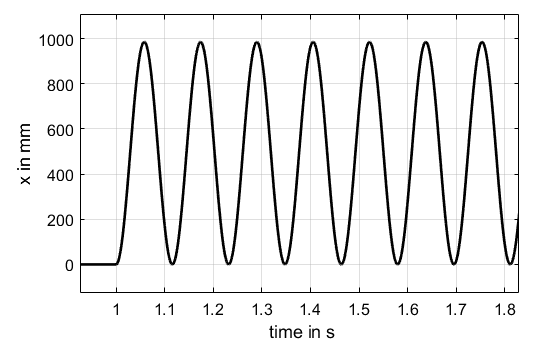
\includegraphics[width=0.45\textwidth]{Bilder/schwingendeStepresponse.png}
	\caption{Sprungantwort der mit mit $K_{P, krit}$ geschlossenen Regelstrecke}
	\label{geschlosseneRegelstreckeP}
\end{figure}

Das Ausgangssignal schwingt dabei mit einer Periodendauer von
$T_{U} = \SI{116}{ms}$. Aus diesen Werten können nun die einzelnen 
Regelparameter berechnet werden.
Nach Ziegler-Nichols berechnen sich die Parameter für
einen PID-Regler in parallel Form nach Tabelle \ref{tbl:PID}.




\begin{table}[hb]

\normalsize

\caption{Parameter-Berechnung nach Ziegler-Nichols mit dem Stabilitätsrandverfahren}

\label{tbl:PID}

\centering

\begin{tabular}{c|c|c|c}

& $K_p$ & $K_i$ & $K_d$\\

\hline

PID & $0.6 \cdot K_{pKrit}$ & $K_p/~(0.5 \cdot T_U)$ & $K_p \cdot 0.12 \cdot T_U$\\

\end{tabular}

\end{table}


Daraus ergeben sich die folgenden Regler-Parameter:

\begin{equation}
	K_{p} = 0.6 \cdot K_{pKrit} = 0.6 \cdot \SI{6,668e6}{} = \SI{4,00e6}{}
\end{equation}

\begin{equation}
	K_{i} = K_p/~(0.5 \cdot T_U) =   \frac{\SI{6,668e6}{} } {0.5 \cdot \SI{116}{ms}} = \SI{115e6}{}
\end{equation}

\begin{equation}
	K_{d} = \SI{6,668e6}{} \cdot 0.12 \cdot \SI{116}{ms} =\SI{92,8e3}{}
\end{equation}

Die berechneten Werte müssen nicht zu zeitdiskreten Parametern umgerechnet werden, da Simulink diese Umrechnung übernimmt.
Die Sprungantwort mit den berechneten Parametern ist in Abbildung \ref{geregelteSprungantwortSchwingend} zu sehen.



\begin{figure}[h] 
	\centering
		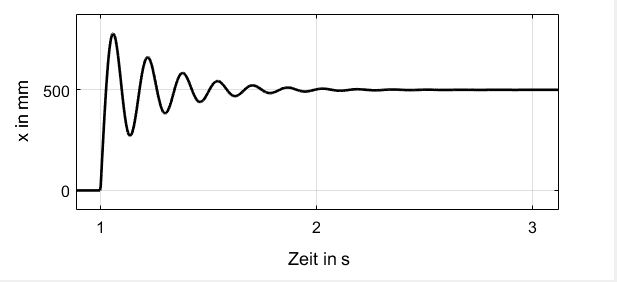
\includegraphics[width=0.45\textwidth]{Bilder/geregelteStepresponseSchwingend.png}
	\caption{mit berechneten Parametern geregelte Sprungantwort}
	\label{geregelteSprungantwortSchwingend}
\end{figure}



\section{Validierung und Verbesserungen}
In diesem Abschnitt wird die Regelung mit den berechneten
Parametern getestet und die Ergebnisse analysiert. Im
Anschluss werden die Parameter so optimiert, dass die
geforderten Projektziele erreicht werden.

Die in Abbildung \ref{geregelteSprungantwortSchwingend} dargestellte regelt recht schnell auf die Wunschhöhe ein.
Jedoch erfüllt dieses Verhalten in keinster Weise die Anforderungen.

\begin{itemize}
	\item Der Überschwinger ist zu groß
	\item Das System schwingt zu stark
	\item Die Beschleunigung ist nicht human
\end{itemize}

Da das Modell als Differenzialgleichung aufgebaut ist, und nicht als eine einzelne Übertragungsfunktion, kann in der Simulation auch die Beschleunigung gemessen werden.
Die Laderaum wird mit bis zu $45g $ beschleunigt.
Dies ist inakzeptabel.

\subsection{Verbesserung durch mauelle Veränderung der Parameter}
Optimalerweise sollte ein Aperiodische Regelverhalten erreicht werden. Ein langsameres einregeln ist nicht nur erlaubt, sogar erwünscht,
da die Ladung nicht durch zu große Beschleunigung belastet werden soll.
Die Annahme ist nun, dass dieses Verhalten durch ein erhöhen des D-Anteils erreicht werden kann.
Dafür wird schrittweise der D-Anteil manuell erhöht und der Effekt analysiert.

Der D-Anteil wird um den Faktor 10 erhöht.

\begin{figure}[h] 
	\centering
		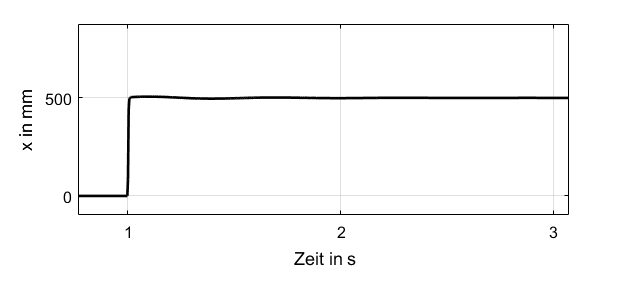
\includegraphics[width=0.45\textwidth]{Bilder/D-Anteilx10.png}
	\caption{geregelte Sprungantwort mit erhöhtem D-Anteil}
	\label{geregelteSprungantwortDx10}
\end{figure}

Die Sprungantwort in \ref{geregelteSprungantwortDx10} sieht schon sehr gut aus.
Der Überschwinger ist maximal und die Wunschwert ist so gut wie sofort erreicht.
Jedoch wird auch mit diesen Parametern wieder eine Beschleunigung von bis zu $200.000 g$ erreicht.
Auch sollte erwähnt werden, dass die eingestellten Parameter des \glqq Simulink-Solver\grqq  für eine solch schnelle Regelung ungeeignet sind.

\begin{itemize}
	\item Solver-Type:   ~~~~~   Fixed-step
	\item Fixed-step size: ~~ $\SI{0,5e-4}{s}$	
\end{itemize}


Mit diesen Parametern wird der Wunschwert in 18 Simulations-Schritten erreicht.

\subsection{Limitierung des Outputs}

Um die Beschleunigung zu limitieren soll die Kraft $F_{s}$ so begrenzt werden, dass die maximale Beschleunigung $0,5 g$ nicht überschreitet.

\begin{equation}
	F_{s, max} = F_{a} = m \cdot a_{max} = \SI{2300}{kg} \cdot \SI{5}{\frac{m}{s^2}} = \SI{11,5}{kN}
\end{equation}

Dieser Wert liegt aber unter dem in \ref{subSec:Interpraetation} berechneten Wert für die minimale Kraft.
Die Kraft wird also auf $F_{s, max} = \SI{100}{kN}$ festgellegt.
Da es sich umn einen Einfach wirkenden Zylinder handelt wird $F_{s, min}$ auf $\SI{0}{kN} $ festgelegt.
Um den Anti-windup Effekt zu verhindern wird im PID-Regler die \glqq Anti-windup Methode\grqq ~ \glqq clamping\grqq ~ aktiviert.


Das System erreicht zwar die gewünschte Position, aber die 
Beschleunigung ist zu groß und das System schwingt enorm. Das limitieren der Stellgröße verändert die dynamik des Systems drastisch.


Das Stabilitätsrandverfahren wird also erneut angewandt. 
Es stellt sich heraus, dass sich  $K_{p, Krit}$ und $T_{U}$ hat sich nicht verändert haben.




\subsection{Wandernder Arbeitspunkt}
Es ergibt sich ein Dilemma:
Die Stellgröße muss limitiert sein, damit die Beschleunigung nicht zu groß ist. 
Aber mit diesem Limitierten Output ist nicht genügend Kraft vorhanden um die Rückstellkraft der Feder zu überwinden und einen Wert, 
auch nur annähernd an der gewünschen Höhe zu erreichen.

Nun ist mir eine Idee gekommen.
Die Beschleunigung des Laderaums und die Überwindung der Feder-Rückstellkraft kann unabhängig voneinander sein.
In jedem beliebigen Arbeitspunkt kann die Kraft der Feder berechnet werden, und auf die Stellgröße oben drauf gerechnet werden.
So kann sich der Regler auf dei Beschleunigung der Masse konzentrieren.

Das Simulink Modell wird, wie in Abbildung \ref{wandernderArbeitspunkt} dargestellt, erweitert:


\begin{figure*}[hbt] 
	\centering
		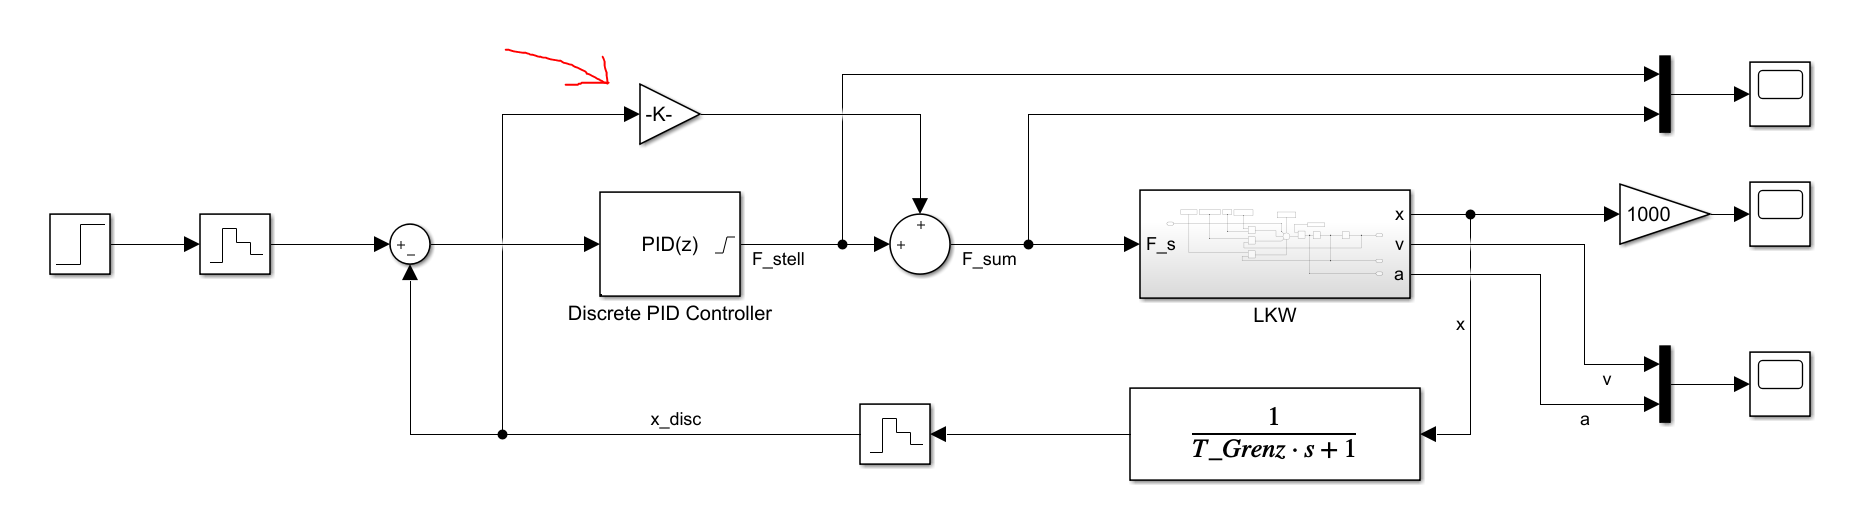
\includegraphics[width=0.95\textwidth]{Bilder/WandernderArbeitspunkt.PNG}
	\caption{Erweitertes Simulink-Modell}
	\label{wandernderArbeitspunkt}
\end{figure*}


Diese Erweiterung übernimmt größtenteils die Arbeit des I-Anteils. Also werden die Regelparameter nochmals nach dem Stabilitätsrandverfahren 
berechnet. Aber diesmal für einen PD-Regler

\begin{table}[hb]

\normalsize

\caption{Parameter-Berechnung nach Ziegler-Nichols mit dem Stabilitätsrandverfahren}

\label{tbl:PID}

\centering

\begin{tabular}{c|c|c|c}

& $K_p$ & $K_i$ & $K_d$\\

\hline

PD & $0.55 \cdot K_{pKrit}$ & $0$ & $K_p \cdot 0.15 \cdot T_U$\\

\end{tabular}

\end{table}


	Durch Ausprobieren wurde herausgefunden, dass die Anti-Windup Methode \glqq back-calculation\grqq  recht gut funktioniert.
	Es wird der Kb koeffizient der \glqq back-calculation\grqq  Methode und der I-Anteil der Reglers so lange angepasst, bis sich
	das System aperiodisch verhält. Die Folgenden Parameter [\ref{eq:finaleParameter}] ergeben ein sehr gutes Regelverhalten (Abbildung \ref{wunderSchoeneSprungantwort}) 


	\begin{equation}
		\label{eq:finaleParameter}
		\begin{split}
		K_p &= \SI{3,67e6}{}\\
		K_i &= \SI{10e6}{}\\
		K_d &= \SI{116e6}{}\\
		\text{Back-calculation coefficient (Kb)} &= 30\\
			\text{Output Saturation}\\
		\text{Upper limit} &= \SI{10}{kN}\\
		\text{Lower limit} &= \SI{-10}{kN}\\
		\end{split}
	\end{equation}


	\begin{figure}[h] 
		\centering
			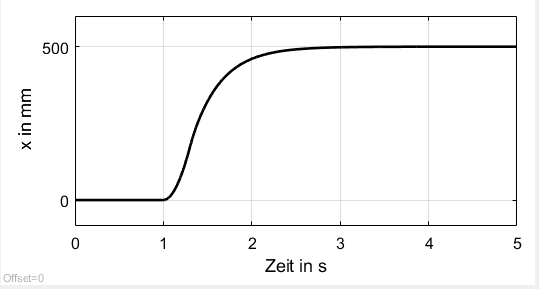
\includegraphics[width=0.45\textwidth]{Bilder/geregelteStepresponseSchoen.PNG}
		\caption{geregelte aperiodische Sprungantwort}
		\label{wunderSchoeneSprungantwort}
	\end{figure}

	Aufgrund der Limitierung der Stellgröße ist für diesen Verlauf (\ref{wunderSchoeneSprungantwort}) auch die Beschleunigung
	human (Abbildung \ref{beschleunigungHuman}).

	\begin{figure}[h] 
		\centering
			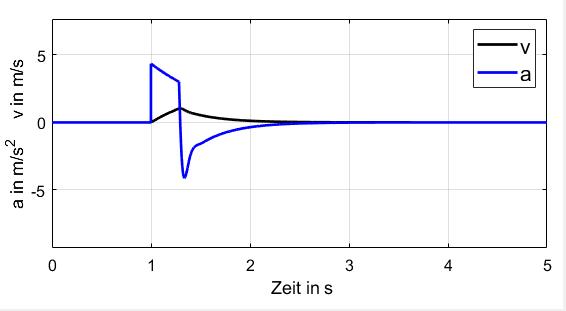
\includegraphics[width=0.45\textwidth]{Bilder/beschleunigungUndGeschwindigkeit.png}
		\caption{Beschleunigung und Geschwindigkeitsverhalten der aperiodischen Regelung}
		\label{beschleunigungHuman}
	\end{figure}

	Es is schön zu sehen, dass der Laderaum erst beschleunigt wird, und gegen Ende dann einmal abnehmend abgebremst wird.
	Dies ist ein annähernd optimales Verhalten.

	





\section{Beobachtungen und andere Effekte}

\section{Schlussfolgerungen}


